% !TeX root = ../main.tex
\chapter{预测}\label{ch6}

第一类应用,例如面部识别、情感分析、对象检测或语音识别,需要从可用信号中预测未知值。

\section{图像去噪}\label{sec6.1}

将深度模型直接应用于图像处理的一个具体应用是利用图像的统计结构中的冗余来从退化中恢复图像。例如,在一张灰度图片中,向日葵的花瓣可以以高置信度进行着色,而几何形状的纹理,例如低光、颗粒状图片上的桌子,可以通过在可能均匀的大区域上进行平均来校正。

\keyterm{去噪自动编码器}是一种模型,它将受损的信号 $\tilde{X}$ 作为输入,并计算出原始信号 $X$ 的估计。对于图像,它是一个可以集成跳跃连接的卷积网络,特别是组合早期获得的相同分辨率的表示 在模型的后期,以及注意层,以方便考虑彼此相距较远的元素。对于图像来说,它是一个卷积网络,可能会集成跳跃连接,尤其是为了组合在模型前期和后期获得的同一分辨率的表示,以及注意力层,以便考虑彼此距离较远的元素。

这样的模型是通过收集大量干净样本及其对应的受损输入来训练的。后者可以在低光或聚焦不足等退化条件下捕获,也可以通过算法生成,例如通过将干净的样本转换为灰度、减小其大小或使用有损压缩方法对其进行激进压缩。

去噪自动编码器的标准训练过程使用所有像素的 MSE 损失之和,在这种情况下,在这种情况下,模型的目标是在给定受损图片的情况下计算出最佳的平均干净图片,即 $E[X \mid \tilde{X}]$。当 $X$ 不完全由 $\tilde{X}$ 确定时,这个量可能是有问题的,在这种情况下,生成信号的某些部分可能是不切实际的、模糊的平均值。

\section{图像分类}\label{sec6.2}

图像\keyterm{分类}是从图像中提取语义的最简单策略,包括在给定输入图像的情况下,从有限的、预定义数量的类别中预测类别。

此任务的标准模型是卷积网络,例如 ResNets(详见 \ref{sec5.2} 节),以及基于注意力的模型,例如 ViT(详见 \ref{sec5.3} 节)。这些模型生成一个 logits 向量,其维度与类别的数量一样多。

训练过程只是最小化交叉熵损失(详见 \ref{sec3.1} 节)。通常,可以通过\keyterm{数据增强}来提高性能,数据增强包括使用手工设计的随机变换修改训练样本,这些变换不会改变图像的语义内容,例如裁剪、缩放、镜像或颜色变化。

\section{对象检测}\label{sec6.3}

图像理解的一个更复杂的任务是\keyterm{对象检测},其目标是在给定输入图像的情况下预测感兴趣对象的类别和位置。

对象位置被形式化为矩形边界框的四个坐标 $(x_1,y_1,x_2,y_2)$,与每个训练图像相关联的真实值是这样的边界框列表,每个边界框都标有其中包含的对象的类别。

解决这一任务的标准方法,例如通过\keyterm{单次检测器}(\keyterm{SSD})\citep{arxiv-1512.02325},是使用卷积神经网络产生一系列大小为 $D_s \times H_s \times W_s$ 的图像表示 $Z_s$,其中 $s = 1, \dots, S$。空间分辨率 $H_s \times W_s$ 逐渐减小,直至 $s = S$ 时缩小为 $1 \times 1$(见图 \ref{fig6.1})。这些张量中的每一个都完全覆盖输入图像,因此 $h,w$ 索引对应于将图像划分为规则正方形,当 $s$ 增加时,规则正方形会变得更加粗糙。

\begin{figure}
    \centering
    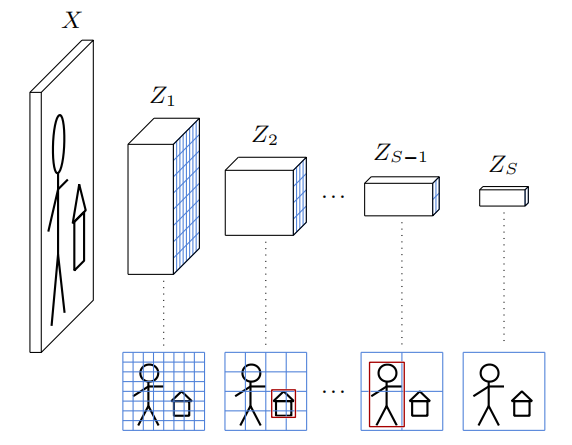
\includegraphics[width=0.9\textwidth]{fig/fig6.1.png}
    \caption[卷积物体检测器]{卷积对象检测器处理输入图像以生成一系列分辨率递减的表示。它在每个尺度 $s$ 上为每个 $h,w$ 计算预定义数量的边界框,这些边界框的中心位于与该单元相对应的图像区域中,并且其大小适合其接受范围。每个预测均采用估计值 ($\hat{x}_1, \hat{x}_2, \hat{y}_1, \hat{y}_2$) 的形式,由上面的红色框表示,以及 $C + 1$ 个 Logits 组成的向量,表示 $C$ 个感兴趣的类别和一个附加的``无对象''类别。}
    \label{fig6.1}
\end{figure}

如 \ref{sec4.2} 节和图 \ref{fig4.4} 所示,由于\keyterm{卷积层}的连续性,特征向量 $(Z_s[0,h,w],\dots,Z_s[D_s-1,h,w])$ 是图像区域的描述符,称为其\keyterm{感受野},它比这个正方形大,但以它为中心。这导致任何边界框 $(x_1,x_2,y_1,y_2)$ 与 $s,h,w$ 的明确匹配,分别由 $\text{max}(x_2-x_1,y_2-y_1), \frac{y_1+y_2}{2}, \frac{x_1+x_2}{2}$ 确定。

检测是通过添加 $S$ 个卷积层来实现的,每个卷积层处理一个 $Z_s$ 并为每个张量索引 $h,w$ 计算边界框的坐标和相关的 logits 值。如果有 $C$ 个对象类别,就会有 $C + 1$ 个 logits 值,额外的一个表示``无对象''。因此,每个附加卷积层都有 $4 + C + 1$ 个输出通道。SSD 算法特别为每个 $s,h,w$ 生成多个边界框,每个边界框专用于硬编码的长宽比范围。

由于使用边界框进行标注需要人工缓慢地干预,因此创建用于对象检测的训练集成本较高。为了缓解这个问题,标准方法是从一个在大型分类数据集上\keyterm{预训练}过的卷积模型开始,比如原始 SSD 使用 VGG-16,然后用额外的卷积层替换其最后的全连接层。令人惊讶的是,尽管对象检测任务涉及到几何量的回归,但仅为分类任务训练的模型所学习到的特征表示却可以重用于对象检测。

在训练过程中,每个真实边界框都与其 $s,h,w$ 相关联,并引入一个损失项,该损失项由 logits 的交叉熵损失和边界框坐标的回归损失(例如 MSE)组成。其他没有边界框匹配的 $s,h,w$ 会引发仅交叉熵惩罚来预测``无对象''类。

\begin{figure}
    \centering
    \includegraphics[width=0.9\textwidth]{fig/fig6.2.png}
    \caption[使用 SSD 进行物体检测]{使用单次检测器进行物体检测的示例 \citep{arxiv-1512.02325}}
    \label{fig6.2}
\end{figure}

\section{语义分割}\label{sec6.4}

\begin{figure}
    \centering
    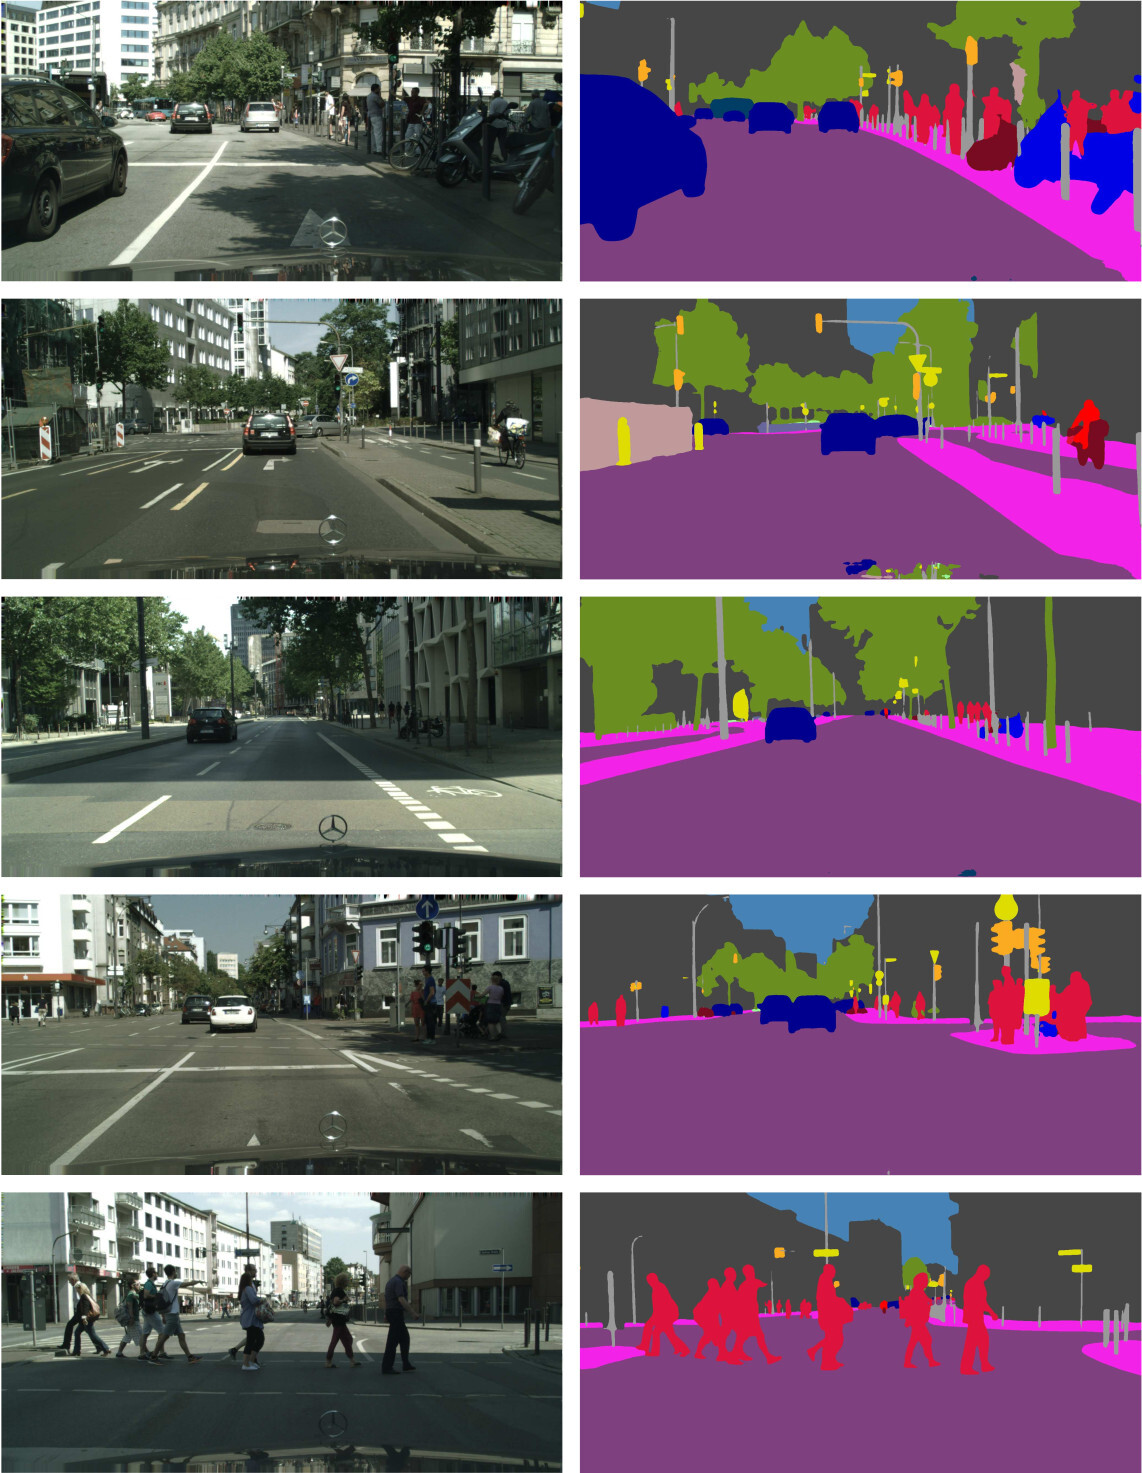
\includegraphics[width=0.9\textwidth]{fig/fig6.3.png}
    \caption[用 PSP 进行语义分割]{金字塔场景分析网络的语义分割结果 \citep{arxiv-1612.01105}}
    \label{fig6.3}
\end{figure}

\section{语音识别}\label{sec6.5}

\section{文本图像表示}\label{sec6.6}

\begin{figure}
    \centering
    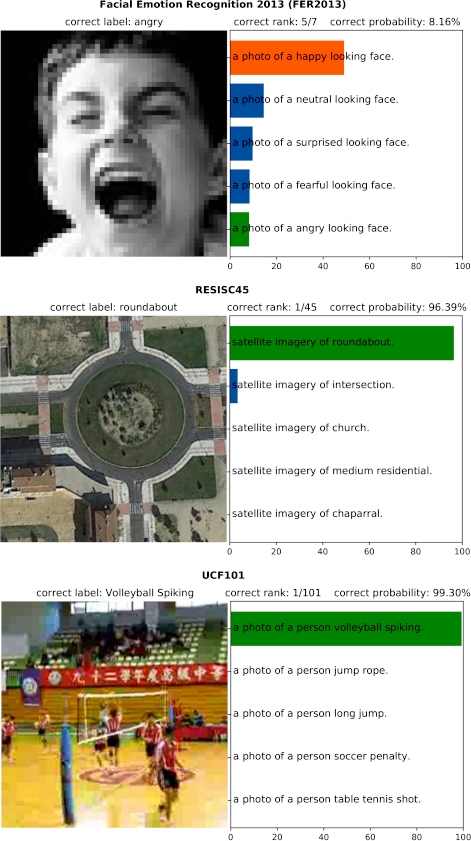
\includegraphics[width=0.9\textwidth]{fig/fig6.4.png}
    \caption[CLIP 零样本预测]{CLIP 文本图像嵌入 \citep{arxiv-2103.00020} 允许通过预测哪类描述嵌入与图像嵌入最一致来进行零样本预测。 }
    \label{fig6.4}
\end{figure}

\section{强化学习}\label{sec6.7}

\begin{figure}
    \centering
    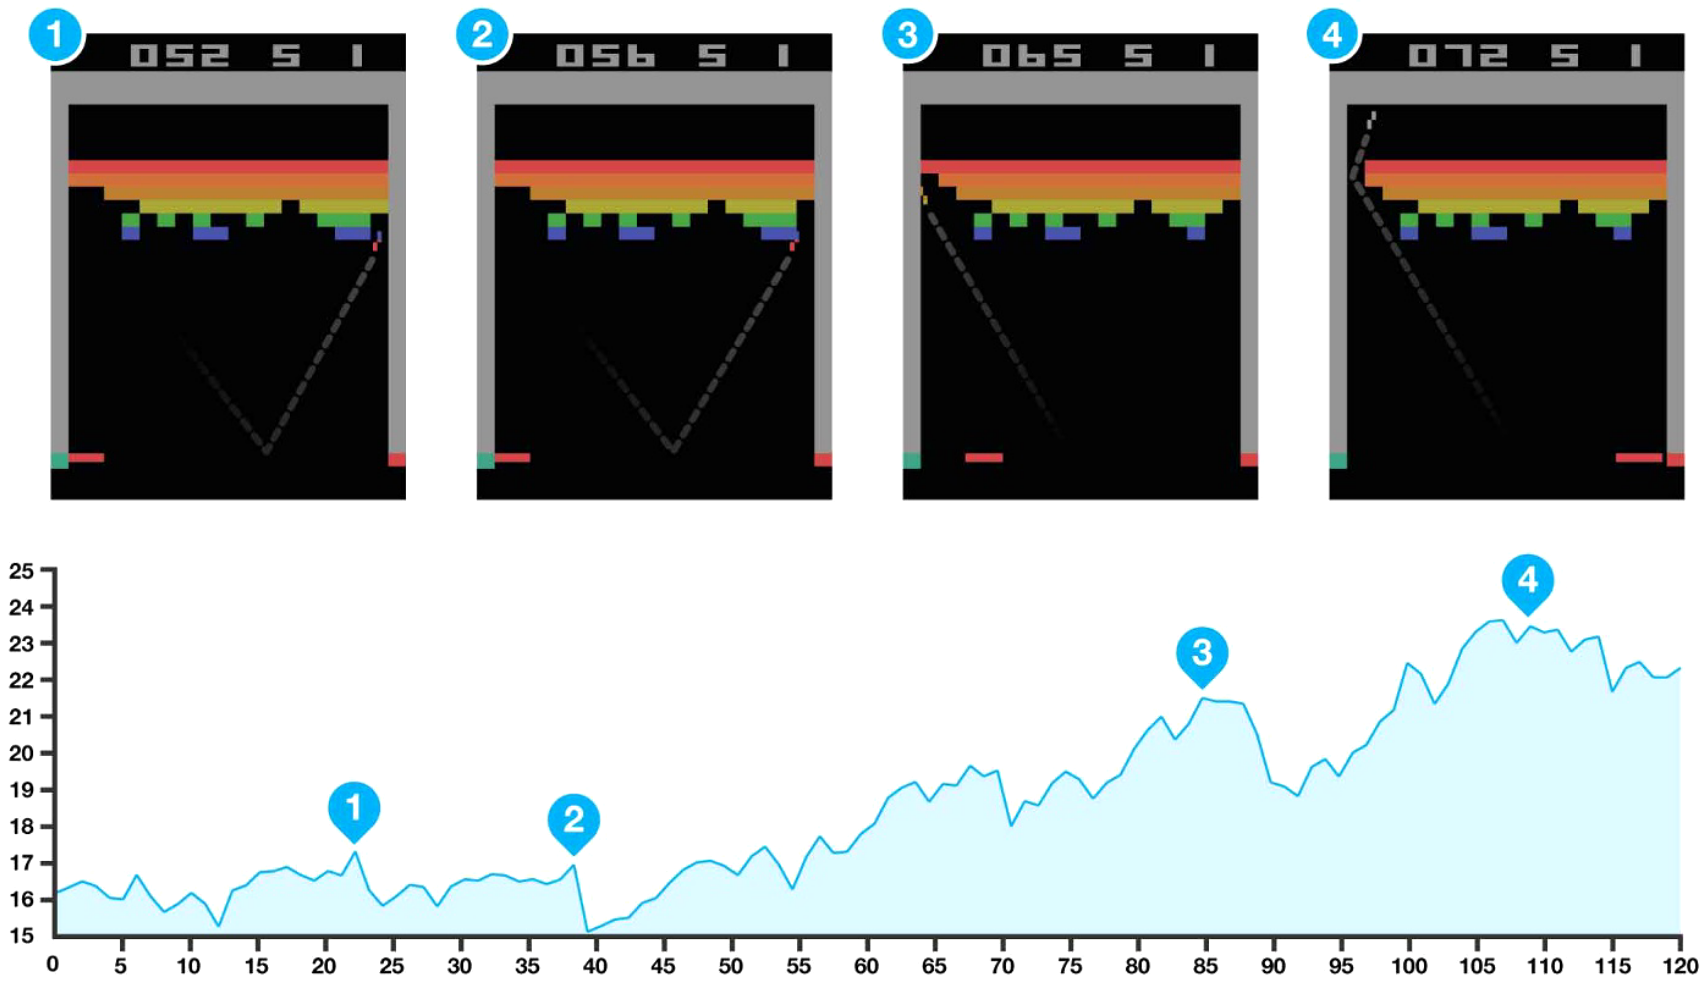
\includegraphics[width=0.9\textwidth]{fig/fig6.5.png}
    \caption[DQN 状态值演化]{该图显示了打砖块游戏期间状态值 $V(S_t)=\max_aQ(S_t,a)$ 的演变。时间点 (1) 和 (2) 处的尖峰对应于清除砖块,在时间点 (3) 处,砖块即将突破顶线,在 (4) 处确实突破了顶线,这确保了未来的高奖励 \citep{nature14236}。}
    \label{fig6.5}
\end{figure}